\chapter{GrShell Language}\indexmain{GrShell}
\label{chapgrshell}

\GrShell\ is a \indexedsee{shell}{GrShell} application of \LibGr\indexmain{libGr}. 
It belongs to \GrG's standard equipment. \GrShell\ is capable of creating, manipulating, and dumping graphs as well as performing and debugging graph rewriting.
The \GrShell\ provides a line oriented scripting language. 
\GrShell\ scripts are structured by simple statements separated by line breaks.

\section{Building Blocks}

\GrShell\ is \indexed{case sensitive}. 
A \indexed{comment} starts with a \indexed{\texttt{\#}} and is terminated by end-of-line or end-of-file. 
Any text left of the \texttt{\#} will be treated as a statement.
The following items are required for representing text, numbers, and rule parameters.\\
\\
\emph{Text}\\
May be one of the following:
\begin{itemize}
  \item A non-empty character sequence consisting of letters, digits, and underscores. The first character must not be a digit.
  \item Arbitrary text enclosed by double quotes (\texttt{""}).
  \item Arbitrary text enclosed by single quotes (\texttt{''}).
\end{itemize}
\mbox{ }\\
\emph{Number}\\
Is an \texttt{int} or \texttt{float} constant in decimal notation (see also Section~\ref{builtin}).

\begin{rail} 
 Parameters : Text + ',' ;
 SpacedParameters: Text + ; 
\end{rail}\ixnterm{Parameters}\ixnterm{SpacedParameters}

In order to describe the commands more precisely, the following (semantic) specializations of \emph{Text} are defined:
\begin{description}
  \item[Filename]A fully qualified file name without spaces (e.g.\ \texttt{/Users/Bob/amazing\textunderscore file.txt}) or a single quoted or double quoted fully qualified file name that may contain spaces (\texttt{"/Users/Bob/amazing file.txt"}).
  \item[Variable] Identifier of a variable that contains a graph element. 
  \item[NodeType, EdgeType] Identifier of a node type resp.\ edge type defined in the model of the current graph.
  \item[AttributeName] Identifier of an attribute.
  \item[Graph] Identifies a graph by its name.
  \item[Action] Identifies a rule by its name.
  \item[Color] One of the following \indexed{color} identifiers: \texttt{Black}, \texttt{Blue}, \texttt{Green}, \texttt{Cyan}, \texttt{Red}, \texttt{Purple}, \texttt{Brown}, \texttt{Grey}, \texttt{LightGrey}, \texttt{LightBlue}, \texttt{LightGreen}, \texttt{LightCyan}, \texttt{LightRed}, \texttt{LightPurple}, \texttt{Yel\-low}, \texttt{White}, \texttt{DarkBlue}, \texttt{DarkRed}, \texttt{DarkGreen}, \texttt{DarkYellow}, \texttt{DarkMagenta}, \texttt{DarkCyan}, \texttt{Gold}, \texttt{Lilac}, \texttt{Turquoise}, \texttt{Aquamarine}, \texttt{Khaki}, \texttt{Pink}, \texttt{Orange}, \texttt{Orchid}. These are the same color identifiers as in \indexed{VCG}/\yComp\ files (for a VCG definition see~\cite{vcg}).
\end{description}
\makeatletter
\begin{rail}
  GraphElement: Text | ('@' '(' Text ')')
\end{rail}\indexmain{\texttt{"@}}\ixnterm{GraphElement}
\makeatother
The elements of a graph (nodes and edges) can be accessed both by their \indexed{variable} identifier and by their \newterm{persistent name} specified through a constructor (see Section~\ref{mani}).
The specializations \emph{Node} and \emph{Edge} of \emph{GraphElement} require the corresponding graph element to be a node or an edge respectively.
\begin{example}
\label{persistentex} 
We insert a node, \indexed{anonymous}ly and with a \indexed{constructor} (see also Section~\ref{mani}):
\begin{grshell}
> select backend lgspBackend.dll
Backend selected successfully.
> new graph "../lib/lgsp-TuringModel.dll" G
New graph "G" of model "Turing" created.
  
# insert an anonymous node... 
# it will get a persistent pseudo name
> new :State  
New node "$0" of type "State" has been created.
> delete node @("$0")
  
# and now with constructor
> new v:State($=start) 
new node "start" of type "State" has been created.
# Now we have a node named "start" and a variable v assigned to "start"
\end{grshell}
\end{example}
\begin{note}
Persistent names belong to a specific graph whereas variables belong to the current \GrShell\ environment. Persistent names will be saved (\texttt{save graph\dots}, see Section~\ref{outputcmds}) and, if you visualize a graph (\texttt{dump graph\dots}, see Section~\ref{outputcmds}), graph elements will be \indexed{label}ed with their persistent names. Persistent names have to be unique for a graph.
\end{note}

\begin{rail}
  Variable '=' GraphElement   
\end{rail}
Assigns the variable or persistent name \emph{GraphElement} to \emph{Variable}. If \emph{Variable} has not been defined yet, it will be defined implicitly. As usual for scripting languages, variables have neither static types nor declarations.

\section{\GrShell\ Commands}
This section describes the \GrShell\ commands. Commands are assembled from basic elements. As stated before commands are terminated by line breaks. Alternatively commands can be terminated by the \indexed{\texttt{;;}} symbol.
\begin{rail}
  Script: ((Command ('<line break>' | ';;'))+) '<end of file>' ;
\end{rail}\ixnterm{Script}

\subsection{Common Commands}
\label{commcommands}
\begin{rail}
  'help'
\end{rail}\ixkeyw{help}
Displays an information message describing supported commands. 

\begin{rail}
  'quit' | 'exit'
\end{rail}\ixkeyw{quit}\ixkeyw{exit}
Quits \GrShell. If \GrShell\ is opened in debug mode, currently active graph viewers (such as \yComp) will be closed as well.

\begin{rail}
  'select' 'backend' Filename ( ( ) | ':' Parameters )
\end{rail}\ixkeyw{select}\ixkeyw{backend}
Selects a \indexed{backend} that handles graph and rule representation. \emph{Filename} has to be a .NET assembly (e.g.\ \texttt{\indexed{lgspBackend.dll}}).
Comma-separated \indexed{parameter}s can be supplied optionally. If so, the backend must support these parameters.

\begin{rail}
  'show' 'backend'
\end{rail}\nopagebreak\ixkeyw{show}\ixkeyw{backend}
List all the parameters supported by the currently selected backend. The parameters can be provided to the \texttt{select backend} command.

\begin{rail}
  'include' Filename
\end{rail}\ixkeyw{include}
Executes the \GrShell\ script\indexmain{graph rewrite script} \emph{Filename}. A \GrShell\ script is just a plain text file containing \GrShell\ commands. They are treated as they would be entered interactively, except for parser errors. If a parser error occurs, execution of the script will stop immediately.

\begin{rail}
  'debug' ( 'enable' | 'disable' )
\end{rail}\ixkeyw{debug}\ixkeyw{enable}\ixkeyw{disable}
Enables and disables the \indexed{debug mode}. The debug mode shows the current working graph in a \yComp\ window. All changes to the working graph are tracked by \yComp\ immediately.  

\begin{rail}
  'debug' 'set' 'layout' (() | Text) ;
\end{rail}\ixkeyw{debug}\ixkeyw{set}\ixkeyw{layout}
Sets the default graph \indexed{layout algorithm} to \emph{Text}. If \emph{Text} is omitted, a list of available layout algorithms is displayed. See Section~\ref{tools:ycomp} on \yComp\ layouters.

\begin{rail}
  'echo' Text
\end{rail}\ixkeyw{echo}
Prints \emph{Text} onto the \GrShell\ command prompt.

\begin{rail}
  '!' CommandLine
\end{rail}\indexmain{\texttt{"!}}
\emph{CommandLine}\indexmain{command line} is an arbitrary text, the operating system attempts to execute.
\begin{example}
On a Linux machine you might execute
\begin{grshell}
!sh -c "ls | grep stuff"
\end{grshell}
\end{example}

\subsection{Graph Commands}
\label{graphcommands}

\begin{rail}
  'new' 'graph' Filename Text 
\end{rail}\ixkeyw{new}\ixkeyw{graph}
Creates a new graph with the model specified in \emph{Filename}\indexmain{graph model}. Its name is set to \emph{Text}. The model file can be either source code (e.g.\ \texttt{turing\textunderscore machineModel.cs}) or a .NET assembly (e.g.\ \texttt{lgsp-turing\textunderscore machineModel.dll}).

\begin{rail}
  'open' 'graph' Filename Text
\end{rail}\ixkeyw{open}\ixkeyw{graph}
Opens the graph \emph{Text} stored in the backend. However, the \emph{LGSPBackend} doesn't support \indexed{persistent graph}s. The \emph{LGSPBackend} is the only backend so far. Therefore this command is currently useless.

\begin{rail}
  'show' 'graphs'
\end{rail}\ixkeyw{show}\ixkeyw{graph}
Displays a list of currently available graphs.

\begin{rail}
  'select' 'graph' Graph
\end{rail}\ixkeyw{select}\ixkeyw{graph}
Selects the current \indexed{working graph}. This graph acts as \emph{\indexed{host graph}} for graph rewrite sequences (see also Sections~\ref{ov:whatsallabout} and~\ref{grsthings}). Though you can define multiple graphs, only one graph can be the active ``working graph''.

\begin{rail}
  'clear' 'graph' (() | Graph)
\end{rail}\ixkeyw{clear}\ixkeyw{graph}
Deletes all graph elements of the current working graph resp.\ the graph \emph{Graph}.

\begin{rail}
  'delete' 'graph' Graph
\end{rail}\ixkeyw{delete}\ixkeyw{graph}
Deletes the graph \emph{Graph} from the backend storage.

\begin{rail}
  'validate' ( ( ) | 'strict' )
\end{rail}\ixkeyw{validate}\ixkeyw{strict}
Validates\indexmain{validate} if the current working graph fulfills the \indexed{connection assertion}s specified in the corresponding graph model. The \emph{strict} mode additionally requires all the edges of the working graph to be specified in order to get a ``valid''. Otherwise edges between nodes without specified constraints are ignored.\\
\begin{example}
We reuse a simplified version of the road map model from chapter~\ref{chapmodellang}:
\begin{grgen} 
model Map;

node class city;
node class metropolis;

edge class street;
edge class highway
      connect metropolis [+] -> metropolis [+];
\end{grgen}
The node constraint on \emph{highway} requires all the metropolises to be connected by highways. Now have a look at the following graph:
\begin{center}
  \fbox{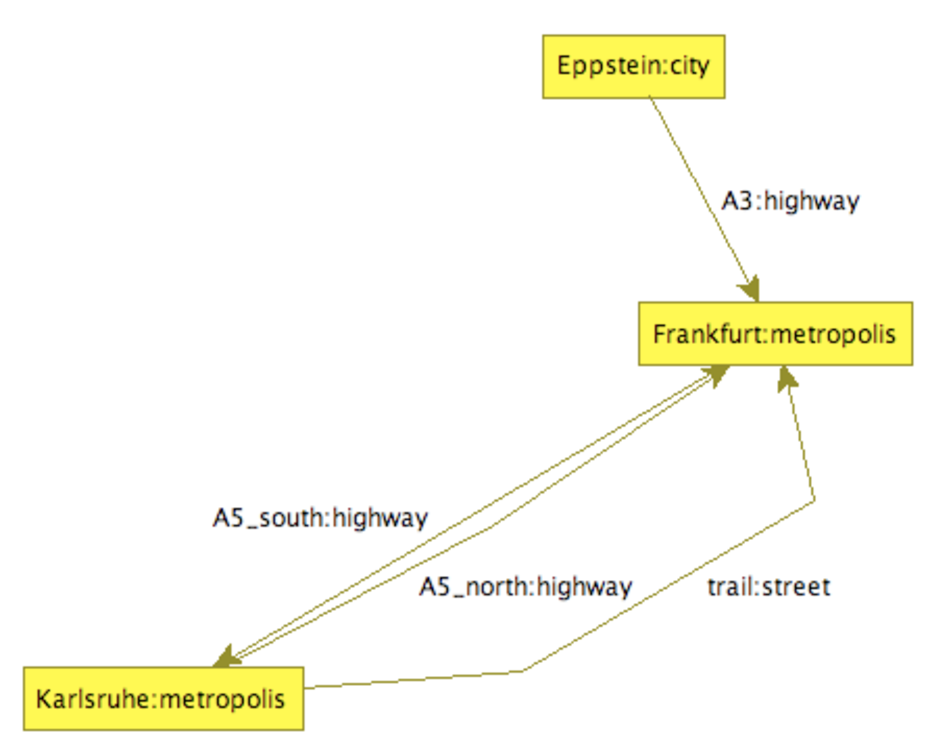
\includegraphics[width=8.5cm]{fig/map}}
\end{center}

This graph is valid but not strict valid.
\begin{grshell} 
> validate
The graph is valid.
> validate strict
The graph is NOT valid:
  CAE: city "Eppstein" -- highway "A3" --> metropolis "Frankfurt" not specified
  CAE: metropolis "Karlsruhe" -- street "trail" --> metropolis "Frankfurt" not specified
>
\end{grshell}
\end{example}

\begin{rail}
  'custom' 'graph' ( ( ) | SpacedParameters )
\end{rail}\ixkeyw{custom}\ixkeyw{graph}
Executes a command specific to the current backend. If \emph{SpacedParameters} is omitted, a list of available commands will be displayed (for the LGSP backend see Sections~\ref{custom}).

\subsection{Graph Manipulation Commands}
\label{mani}
Graph manipulation commands alter existing graphs including creating and deleting graph elements and setting attributes.

\begin{rail}
  Constructor : '(' (() | (dollar '=' Text (() | ',' Attributes) | Attributes)) ')';
  Attributes : AttributeName '=' (Text | Number) + ',' ;
\end{rail}\indexmain{\texttt{\$}}\ixnterm{Constructor}\ixnterm{Attributes}
A \indexed{constructor} is used to initialize a new graph element (see \texttt{new \dots} below). A comma separated list of \indexed{attribute} declarations is supplied to the constructor. Available attribute names are specified by the graph model of the current working graph. All the undeclared attributes will be initialized with \indexed{default value}s, depending on their type (int $\leftarrow$ \texttt{0}, enum $\leftarrow$ unspecified; boolean $\leftarrow$ \texttt{false}; float, double $\leftarrow$ \texttt{0.0}; string $\leftarrow$ \texttt{""}).\\
The \texttt{\$} is a special attribute name: a unique identifier of the new graph element. This identifier is also called \newterm{persistent name} (see Example~\ref{persistentex}). This name can be specified by a constructor only.

\begin{rail}
  'new' (() | Text) (() | ':' NodeType (() | Constructor))
\end{rail}\ixkeyw{new}
Creates a new node within the current graph. Optionally a variable \emph{Text} is assigned to the new node. If \emph{NodeType} is supplied, the new node will be of type \emph{NodeType} and attributes can be initialized by a constructor. Otherwise the node will be of the base node class type \emph{Node}.
\begin{note}
The \GrShell\ can reassign \indexed{variable}s. 
This is in contrast to the rule language (chapter~\ref{chaprulelang}), where we use \emph{\indexed{names}}.
\end{note}

\begin{rail}
  'new' Node '-' (()|Text) \\ (() | ':' EdgeType (() | Constructor)) '->' Node
\end{rail}\ixkeyw{new}
Creates a new edge within the current graph between the specified nodes, directed towards the second \emph{Node}. Optionally a variable \emph{Text} is assigned to the new edge. If \emph{EdgeType} is supplied, the new edge will be of type \emph{EdgeType} and attributes can be initialized by a constructor. Otherwise the edge will be of the base edge class type \emph{Edge}.

\begin{rail}
  GraphElement '.' AttributeName '=' (Text | Number) ;
\end{rail}
Set the \indexed{attribute} \emph{AttributeName} of the graph element \emph{GraphElement} to the value of \emph{Text} or \emph{Number}.

\begin{rail}
  'delete' 'node' Node
\end{rail}\ixkeyw{delete}\ixkeyw{node}
Deletes the node \emph{Node} from the current graph. Incident edges will be deleted as well.

\begin{rail}
  'delete' 'edge' Edge
\end{rail}\ixkeyw{delete}\ixkeyw{edge}
Deletes the edge \emph{Edge} from the current graph.
  
\subsection{Graph Query Commands}

\begin{rail}
  'show' (() | 'num') ('nodes' (() | (() | 'only') NodeType) | 'edges' (() | (() | 'only') EdgeType))
\end{rail}\ixkeyw{show}\ixkeyw{num}\ixkeyw{nodes}\ixkeyw{edges}\ixkeyw{only}
Gets the \indexed{persistent name}s and the types of all the nodes/edges of the current graph. 
If a node type or edge type is supplied, only elements compatible to this type are considered. 
The \texttt{only} keyword excludes subtypes. Nodes/edges without persistent names are shown with a pseudo-name.
If the command is specified with \texttt{num}, only the number of nodes/edges will be displayed.

\begin{rail}
  'show' ('node' | 'edge') 'types'
\end{rail}\ixkeyw{show}\ixkeyw{node}\ixkeyw{edge}
Gets the node/edge types of the current graph model.

\begin{rail}
'show' ('node' ('super' | 'sub') 'types' NodeType | 'edge' ('super' | 'sub') 'types' EdgeType)
\end{rail}\ixkeyw{show}\ixkeyw{node}\ixkeyw{edge}\ixkeyw{super}\ixkeyw{sub}\indexmain{inheritance}
Gets the inherited/descendant types of \emph{NodeType}/\emph{EdgeType}.

\begin{rail}
  'show' ('node' 'attributes' (() | (() | 'only') NodeType) | 'edge' 'attributes' (() | (() | 'only') EdgeType))
\end{rail}\ixkeyw{show}\ixkeyw{node}\ixkeyw{edge}\ixkeyw{only}
Gets the available node/edge \indexed{attribute} types. If \emph{NodeType}/\emph{EdgeType} is supplied, only attributes defined in \emph{NodeType}/\emph{EdgeType} are diplayed. The \texttt{only} keyword excludes inherited attributes.\\
\begin{note}
The \texttt{show nodes/edges attributes\dots} command covers types and \emph{inherited} types. This is in contrast to the other \texttt{show\dots} commands where types and \emph{sub}types are specified or the direction in the type hierarchy is specified explicitly, respectively.
\end{note}

\begin{rail}
 'show' ('node' Node | 'edge' Edge)
\end{rail}\ixkeyw{show}\ixkeyw{node}\ixkeyw{edge}
Gets the attribute types and values of a specific graph element.

\begin{rail}
  'show' GraphElement '.' AttributeName
\end{rail}\ixkeyw{show}
Gets the value of a specific attribute.

\begin{rail}
  'node' 'type' Node 'is' Node | 'edge' 'type' Edge 'is' Edge
\end{rail}\ixkeyw{node}\ixkeyw{edge}\ixkeyw{type}\ixkeyw{is}
Gets the information whether the first element is \indexed{type-compatible}\indexmainsee{compatible types}{type-compatible} to the second element.

\subsection{Graph Output Commands}
\label{outputcmds}

\begin{rail}
  'save' 'graph' Filename
\end{rail}\ixkeyw{save}\ixkeyw{graph}
Dumps\indexmain{dumping graph} the current graph as \GrShell\ script\indexmain{graph rewrite script} into \emph{Filename}. The created script includes
\begin{itemize}
  \item selecting the backend
  \item creating all nodes and edges
  \item restoring the persistent names (see Section~\ref{mani})
\end{itemize}
but not necessarily using the same commands you typed in during construction. 
Such a script can be loaded and executed by the \texttt{include} command (see Section~\ref{commcommands}).

\begin{rail}
  'show' 'graph' Filename (() | Text)
\end{rail}\ixkeyw{show}\ixkeyw{graph}
Dumps the current graph as \indexed{VCG} formatted file into a temporary file. \emph{Filename} specifies an executable. The temporary VCG file will be passed to \emph{Filename} as last parameter. Additional parameters, such as program options, can be specified by \emph{Text}. If you use \yComp\footnote{See Section~\ref{tools:ycomp}.}\indexmain{yComp} as executable, this may look like
\begin{center}
  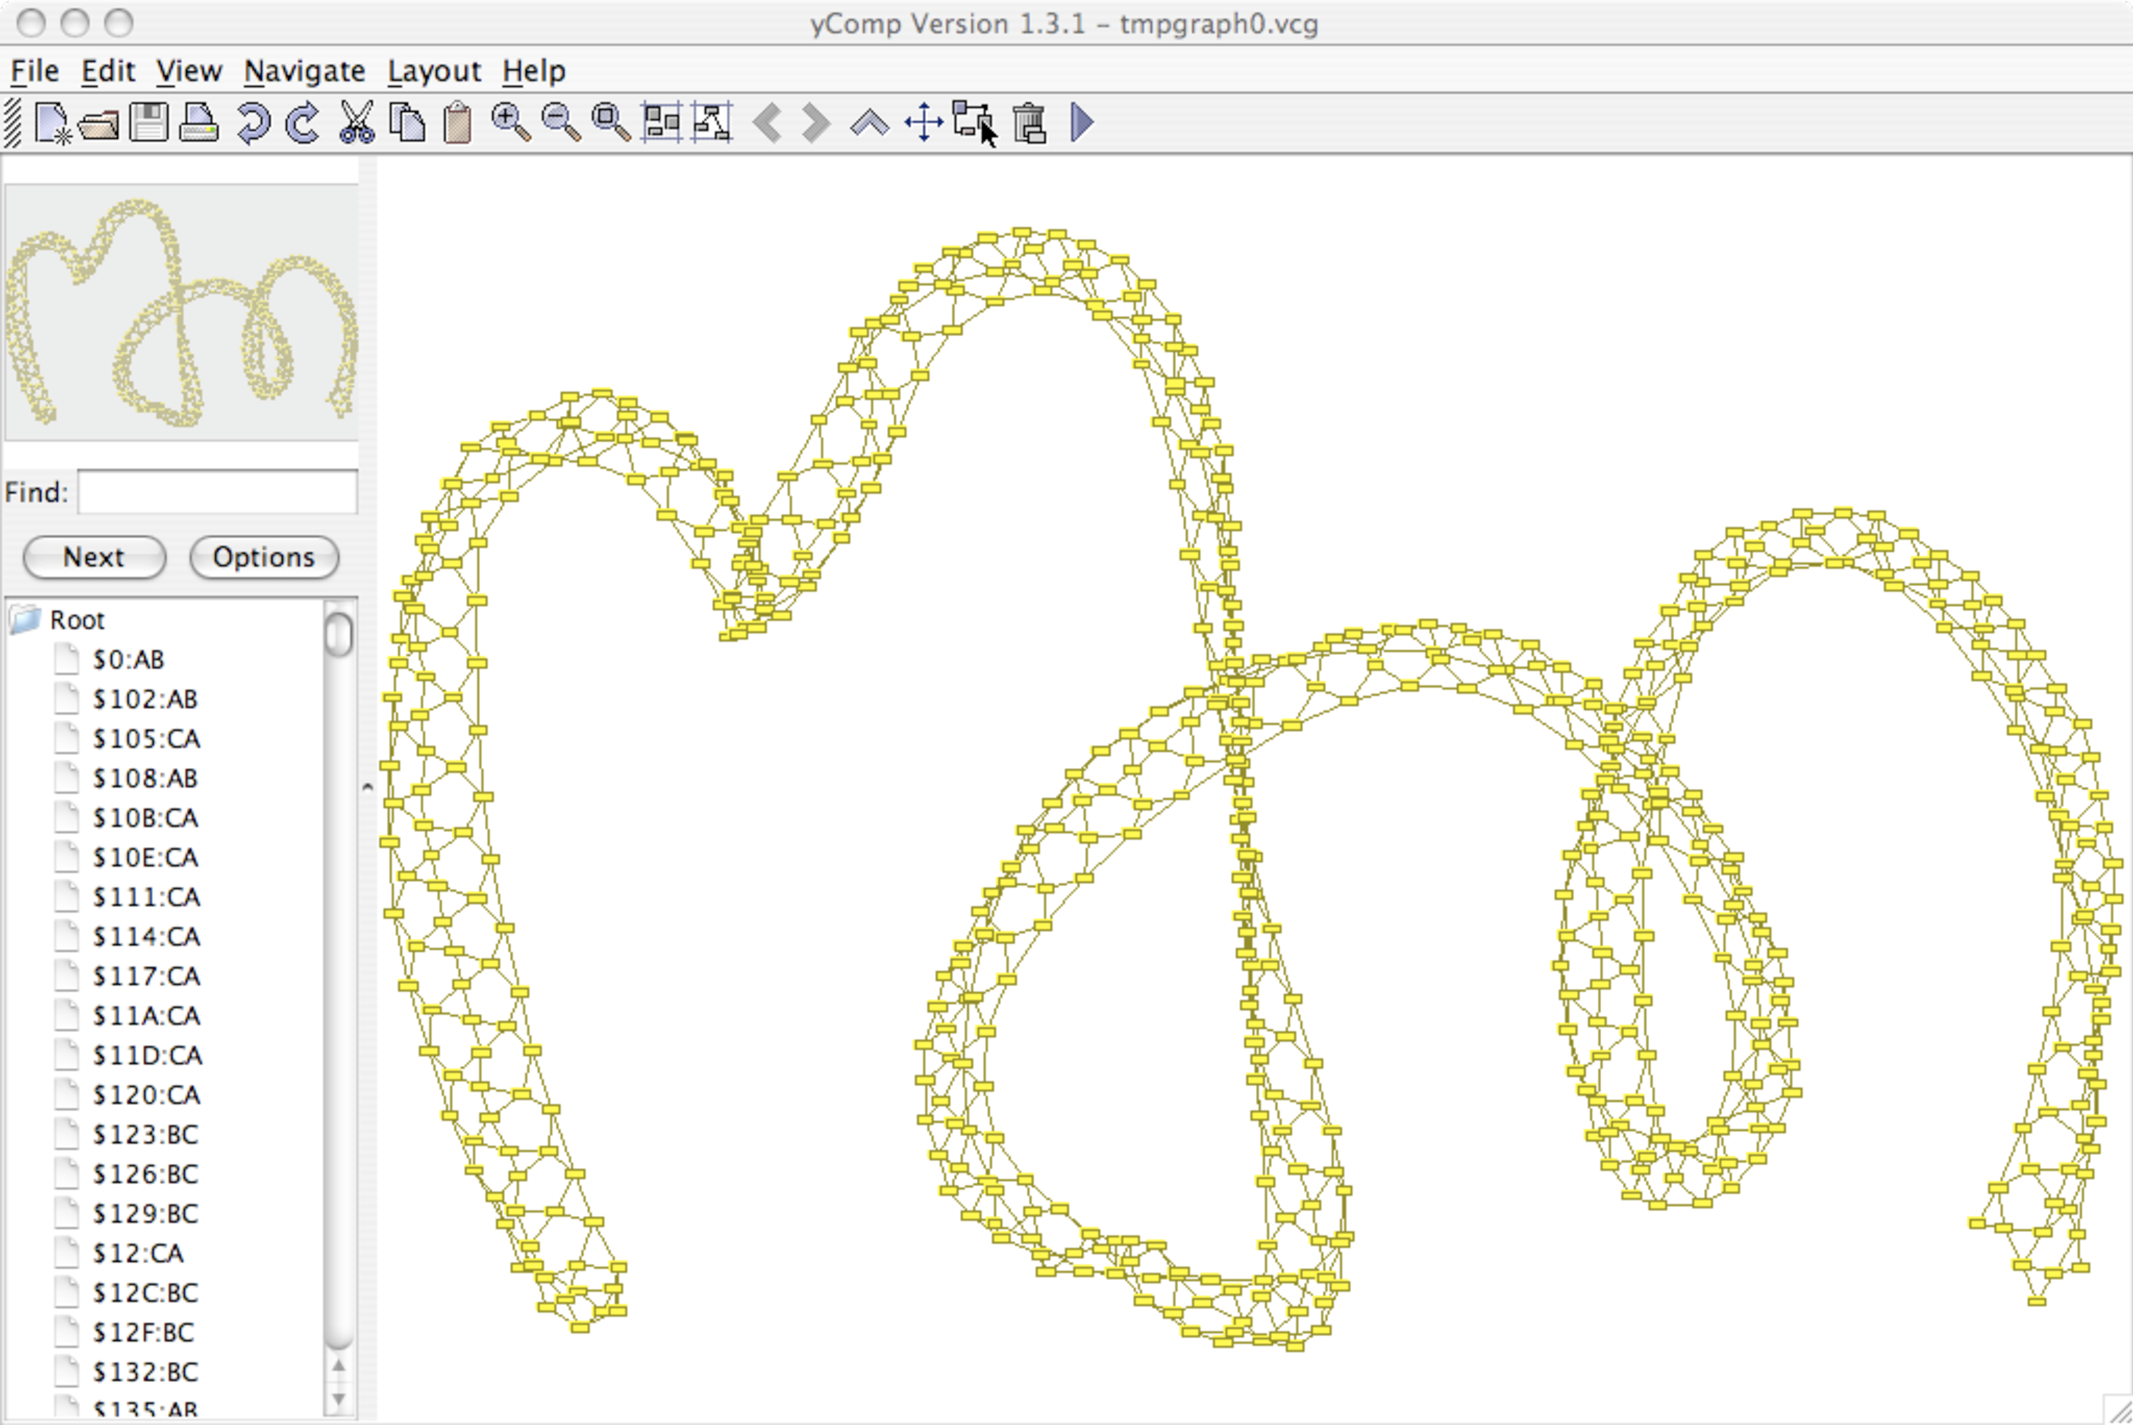
\includegraphics[width=0.75\linewidth]{fig/showgraph}
\end{center}  
The temporary file will be deleted, when the application \emph{Filename} is terminated if \GrShell\ is still running at this time.

\begin{rail}
  'dump' 'graph' Filename
\end{rail}\ixkeyw{dump}\ixkeyw{graph}
Dumps the current graph in \indexed{VCG} format into the file \emph{Filename}.\\

\paragraph{Visualization Styles}
The following commands control the style of the VCG output. This affects \texttt{dump graph}, \texttt{show graph}, and \texttt{enable debug}. 
\begin{rail}
  'dump' 'set' 'node' (() | 'only') NodeType \\ (('color' | 'textcolor' | 'bordercolor') Color | 'shape' Text) ;
\end{rail}\ixkeyw{dump}\ixkeyw{set}\ixkeyw{node}\ixkeyw{only}\ixkeyw{color}\ixkeyw{textcolor}\ixkeyw{bordercolor}\ixkeyw{shape}
Sets the \indexed{color}, text color, border color, or the shape of the nodes of type \emph{NodeType} and all of its subtypes. The keyword \texttt{only} excludes the subtypes. The following shapes are supported: \texttt{box}, \texttt{triangle}, \texttt{circle}, \texttt{ellipse}, \texttt{rhom}, \texttt{hexagon}, \texttt{trapeze}, \texttt{uptrapeze}, \texttt{lparallelogram}, \texttt{rparallelogram}. Those are shape names of \yComp\ (for a VCG definition see~\cite{vcg}).

\begin{rail}
  'dump' 'set' 'edge' (() | 'only') EdgeType ('color' | 'textcolor') Color ;
\end{rail}\ixkeyw{dump}\ixkeyw{set}\ixkeyw{edge}\ixkeyw{only}\ixkeyw{color}\ixkeyw{textcolor}
Sets the color or text color of the edges of type \emph{EdgeType} and all of its subtypes. The keyword \texttt{only} excludes the subtypes.

\begin{rail}
  'dump' 'add' 'node' (() | 'only') NodeType 'exclude' ;
\end{rail}\ixkeyw{dump}\ixkeyw{add}\ixkeyw{node}\ixkeyw{only}\ixkeyw{exclude}
Excludes nodes of type \emph{NodeType} and all of its subtypes as well as their incident edges from output. The keyword \texttt{only} excludes the subtypes, i.e.\ subtypes of \emph{NodeType} are dumped.

\begin{rail}
  'dump' 'add' 'node' NodeType 'group' ;
\end{rail}\ixkeyw{dump}\ixkeyw{add}\ixkeyw{node}\ixkeyw{group}
Declares \emph{NodeType} and subtypes of \emph{NodeType} as \indexed{group node} type. All the differently typed nodes that point to a node of type \emph{NodeType} (i.e.\ there is a directed edge between such nodes) will be grouped and visibly enclosed by the \emph{NodeType}-node.
The following example shows \emph{metropolis} ungrouped and grouped:
\begin{center}
  \fbox{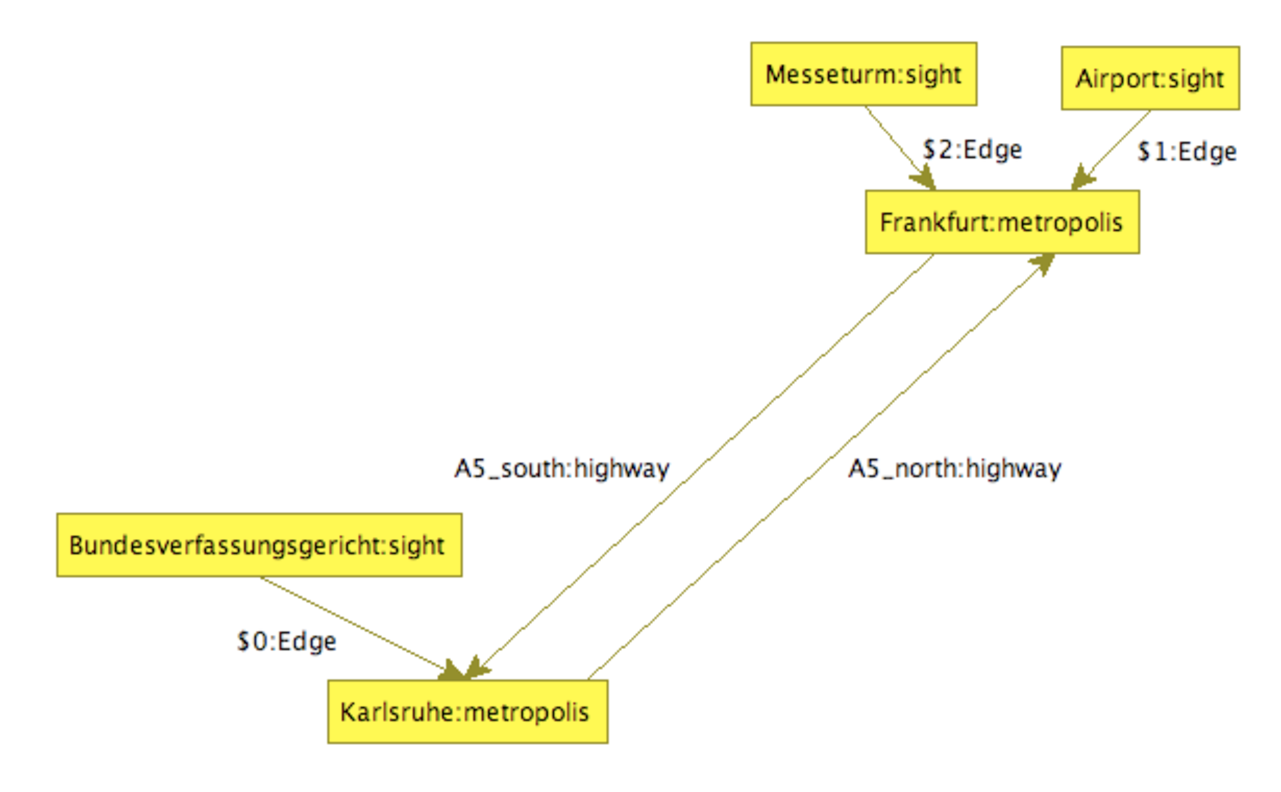
\includegraphics[width=0.45\linewidth]{fig/group2-1}}  \hfill \fbox{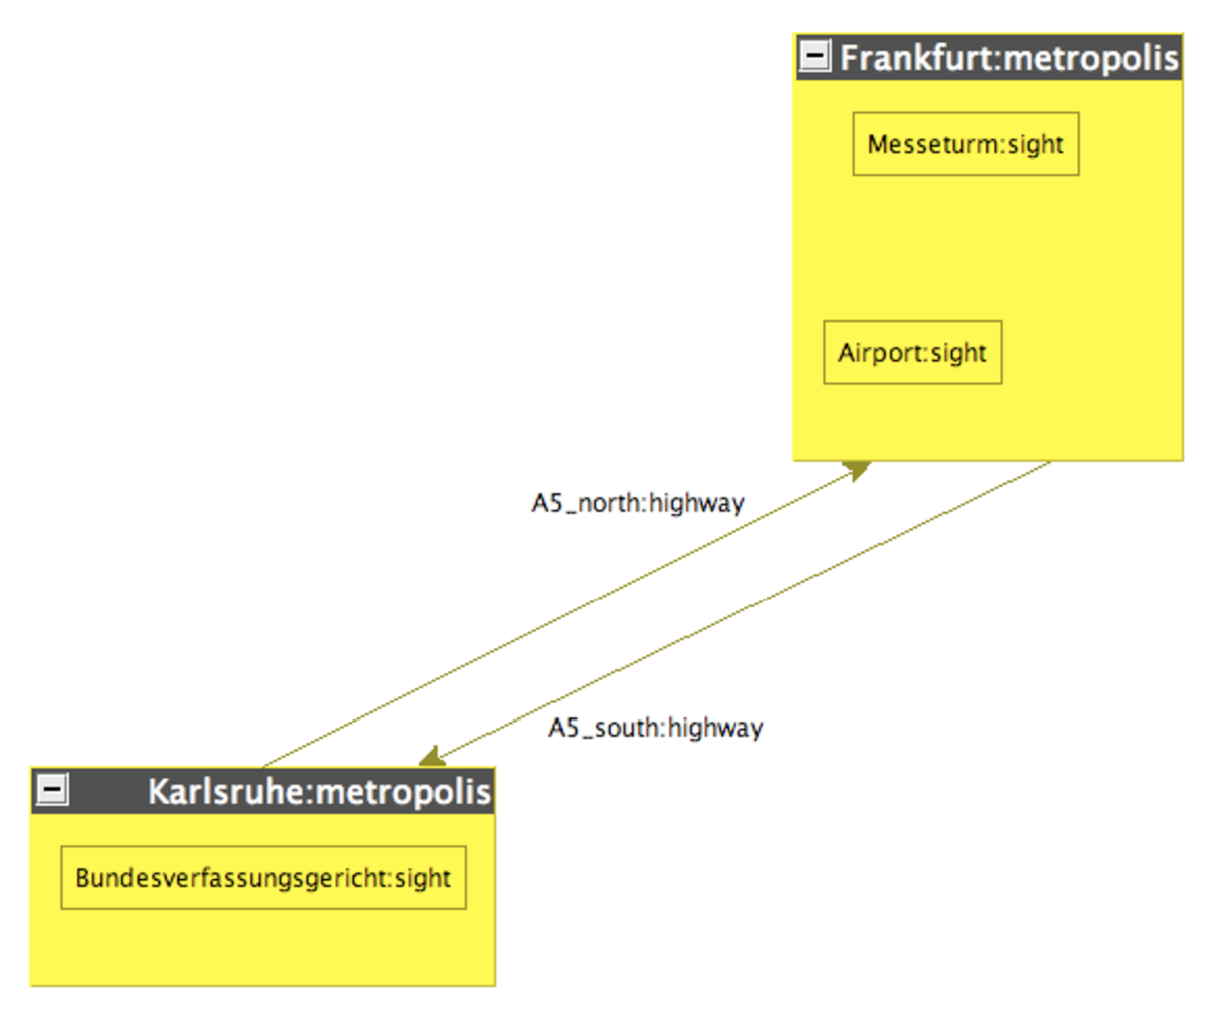
\includegraphics[width=0.45\linewidth]{fig/group2-2}}\\
  {\small right side: dumped with \texttt{dump add node metropolis group}}
\end{center}

\begin{rail}
  'dump' 'add' (() | 'only') ('node' NodeType | 'edge' EdgeType) \\ 'infotag' AttributeName
\end{rail}\ixkeyw{dump}\ixkeyw{add}\ixkeyw{only}\ixkeyw{node}\ixkeyw{edge}\ixkeyw{infotag}
Declares the \indexed{attribute} \emph{AttributeName} to be an ``\indexed{info tag}''. Info tags are displayed like additional node/edge \indexed{label}s. The keyword \texttt{only} excludes the subtypes of \emph{NodeType} resp.\ \emph{EdgeType}. In the following example \emph{river} and \emph{jam} are info tags:
\begin{center}
  \fbox{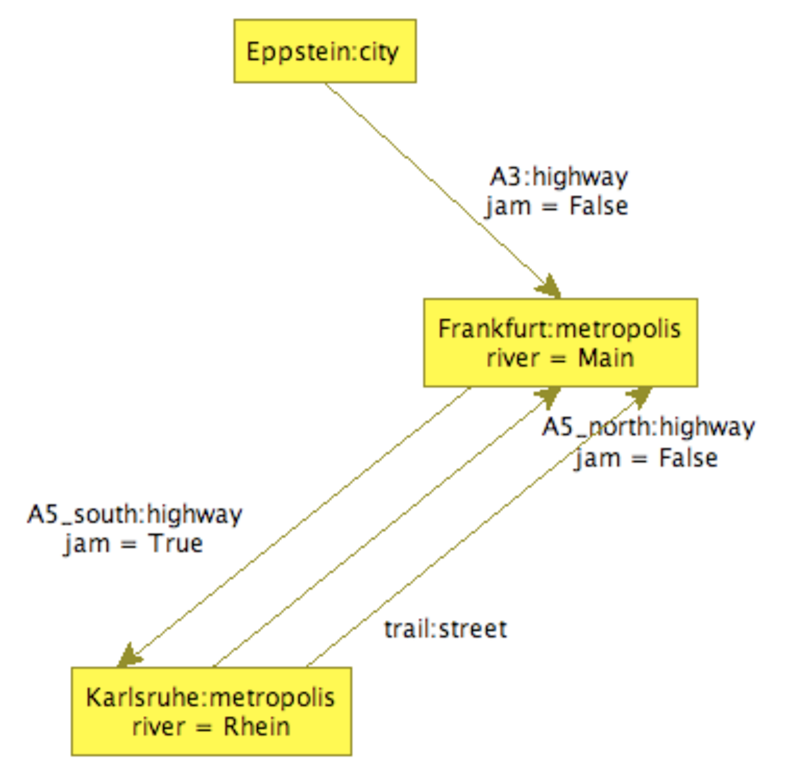
\includegraphics[width=0.5\linewidth]{fig/infotag}}
\end{center}


\begin{rail}
  'dump' 'set' 'edge' 'labels' ('on' | 'off')
\end{rail}\ixkeyw{dump}\ixkeyw{set}\ixkeyw{edge}\ixkeyw{labels}\ixkeyw{on}\ixkeyw{off}
Specifies whether edge \indexed{label}s will be displayed or not (defaults to ``on'').

\begin{rail}
  'dump' 'reset'
\end{rail}\ixkeyw{dump}\ixkeyw{reset}
Reset all style options (\texttt{dump set}\dots) to their default values.

\subsection{Action Commands (GRS)}\indexmain{action command}\indexmainsee{action}{graph rewrite sequence}
\label{grsthings}
An \emph{action} denotes a graph rewrite rule.

\begin{rail}
  'select' 'actions' Filename
\end{rail}\ixkeyw{select}\ixkeyw{actions}
Selects a \indexed{rule set}. \emph{Filename} can either be a .NET assembly (e.g.\ ``rules.dll'') or a source file (``rules.cs''). Only one rule set can be loaded simultaneously.

\begin{rail}
  'show' 'actions'
\end{rail}\ixkeyw{show}\ixkeyw{actions}
Lists all the rules of the loaded rule set, their parameters, and their return values. Rules can return a set of graph elements.

\begin{rail}
  'custom' 'actions' (() | SpacedParameters)
\end{rail}\ixkeyw{custom}\ixkeyw{actions}
Executes an action specific to the current \indexed{backend}. If \emph{SpacedParameters} is omitted, a list of available commands will be displayed (for the LGSPBackend see Section~\ref{custom}).

\makeatletter
\begin{rail}
  GraphRewriteSequence: (() | 'debug') 'grs' SimpleRewriteSequence ;
\end{rail}\ixkeyw{debug}\ixkeyw{grs}\indexmain{graph rewrite sequence}\indexmainsee{GRS}{graph rewrite sequence}\ixnterm{GraphRewriteSequence}
This executes the graph rewrite sequence \emph{SimpleRewriteSequence}.
\begin{rail}
  SimpleRewriteSequence: (SimpleTerm (() | ('*' | lbrace Number rbrace))) + ((() | dollar) (';' | '|' | ampersand));
  SimpleTerm: (() | '!') ('[' Rule ']' | Rule) |
    Text '=' (Text | '@' '(' Text ')') |
    'def' '(' Parameters ')' |
    'true' |
    'false' |
    '(' SimpleRewriteSequence ')' ;
  Rule: (() | '(' Parameters ')' '=') Action (() | '(' Parameters ')') ;
\end{rail}\ixnterm{SimpleRewriteSequence}\ixnterm{SimpleTerm}
\makeatother
\mbox{\quad}\\
Table~\ref{ruletab} lists graph rewrite expressions at a glance. The operators hold the following \indexed{order of precedence}, starting with the lowest priority: 
\[ \text{\texttt{;}} \;\;\;\;\;\;\; \text{\texttt{|}} \;\;\;\;\;\;\;  \text{\texttt{\&}}\] 
\makeatletter
\begin{table}[htbp]
\begin{minipage}{\linewidth} \renewcommand{\footnoterule}{} 
\begin{tabularx}{\linewidth}{|lX|}
\hline
\texttt{s ; t}		& \textbf{Concatenation.} First execute \texttt{s} afterwards execute \texttt{t}. The sequence \texttt{s ; t} is \emph{successfully} executed iff \texttt{s} or \texttt{t} is successfully executed.\\
\texttt{s | t}		& \textbf{XOR.} First execute \texttt{s}. Only if \texttt{s} fails (i.e. can not be executed successfully) then execute \texttt{t}. The sequence \texttt{s | t} is successfully executed iff \texttt{s} or \texttt{t} is successfully executed.\\
\texttt{s \& t}	& \textbf{Transactional AND.} First execute \texttt{s}, afterwards execute \texttt{t}. If \texttt{s} or \texttt{t} fails, the action will be terminated and a rollback to the state before \texttt{s \& t} is performed.\\
\texttt{\$<op>}	& Flag the operator \texttt{<op>} as commutative. Usually operands are executed/evaluated from left to right with respect to bracketing (left-\indexed{associative}). But the sequences \texttt{s}, \texttt{t}, \texttt{u} in \texttt{s \$<op> t \$<op> u} are executed/evaluated in arbitrary order. \\
\texttt{s *}		& Execute \texttt{s} repeatedly as long as its execution does not fail.\\
\texttt{s \{n\}}	& Execute \texttt{s} repeatedly as long as its execution does not fail but \texttt{n} times at most.\\
\texttt{!}		& Dump found matches into VCG formatted files (for a VCG definition see~\cite{vcg}). Every match produces three files within the current directory:
\begin{enumerate}
  \item The complete graph that has the matched graph elements marked
  \item The complete graph with additional information about matching details
  \item A subgraph containing only the matched graph elements
\end{enumerate}\\
\texttt{\emph{Rule}} & Rewrite the first found pattern match produced by the action \emph{Rule}.\\
\texttt{[\emph{Rule}]} & Rewrite every pattern match produced by the action \emph{Rule}. \textbf{Note:} This operator is mainly added for benchmark purposes. Its semantics is not equal to \texttt{Rule*}. Instead this operator collects all the matches first before starting rewritings. In particular one needs to avoid deleting a graph element that is bound by another match. \\
\texttt{v = w}	& Assign the variable \texttt{w} to \texttt{v}. If \texttt{w} is undefined, \texttt{v} will be undefined, too.\\
\texttt{v = @(x)}	& Assign the graph element identified by \texttt{x} to the variable \texttt{v}. If \texttt{x} is not defined, \texttt{v} will be undefined, too.\\
\texttt{def(\emph{Parameters})} & Is \emph{successful} if all the graph elements in \emph{Parameters} exist, i.e.\ if all the variables are defined.\\
\texttt{true}	& A constant acting as a successful match.\\
\texttt{false}	& A constant acting as a failed match.\\ \hline
\end{tabularx}\indexmain{\texttt{;}}\indexmain{\texttt{\&\&}@\texttt{"|}}
\indexmain{\texttt{\&}}\indexmain{\texttt{\$<op>}}\indexmain{\texttt{*}}\indexmain{\texttt{"!}}
\ixkeyw{def}
\end{minipage}\\
\\ 
{\small Let \texttt{s}, \texttt{t}, \texttt{u} be graph rewrite sequences, \texttt{v}, \texttt{w} variable identifiers, \texttt{x} an identifier of a graph element, \texttt{<op>} $\in \{\texttt{;}, \texttt{|}, \texttt{\&}\}$ and \texttt{n} $\in \N_0$.}
\caption{Graph rewrite expressions}
\label{ruletab}
\end{table}
\makeatother

Graph elements returned by rules can be assigned to variables\indexmain{variable} using \texttt{(Para\-meters) = \emph{Action}}\indexmain{parameter}. 
The desired variable identifiers have to be listed in \emph{Parameters}. 
Graph elements required by rules must be provided using \texttt{Action (Para\-meters)}, where \emph{Parameters} is a list of variable identifiers. 
For \indexed{undefined variables} see Section~\ref{ruledecls}, \emph{Parameters}.

Use the \texttt{debug}\indexmain{debugger} option to trace the rewriting process step-by-step. During execution \yComp\footnote{Make sure, that the path to your \texttt{\indexed{yComp.jar}} package is set correctly in the \texttt{ycomp} shell script within \GrG's \texttt{/bin} directory.}\indexmain{yComp} will display every single step. The debugger can be controlled by \GrShell. The debug commands are shown in Table~\ref{tabdebug}.\\
\begin{table}[htbp]
  \begin{tabularx}{\linewidth}{|lX|} \hline
  \texttt{s}(tep) & Execute the next rewrite rule (match and rewrite)\\
  \texttt{d}(etailed step) & Execute a rewrite rule in a three-step procedure: matching, highlighting elements to be changed, doing rewriting \\
  \texttt{n}(ext) & Ascend one level up within the \indexed{Kantorowitsch tree} of the current rewrite sequence (see Example~\ref{ex:debug})\\
  (step) \texttt{o}(ut) & Continue a rewrite sequence until the end of the current loop. If the execution is not in a loop at this moment, the complete sequence will be executed\\
  \texttt{r}(un) &  Continue execution without further stops\\
  \texttt{a}(bort) & Cancel the execution immediately\\ \hline 
  \end{tabularx}
  \caption{\GrShell\ debug commands}
  \label{tabdebug}
\end{table}
%\begin{figure}[htbp]
%  \centering
%  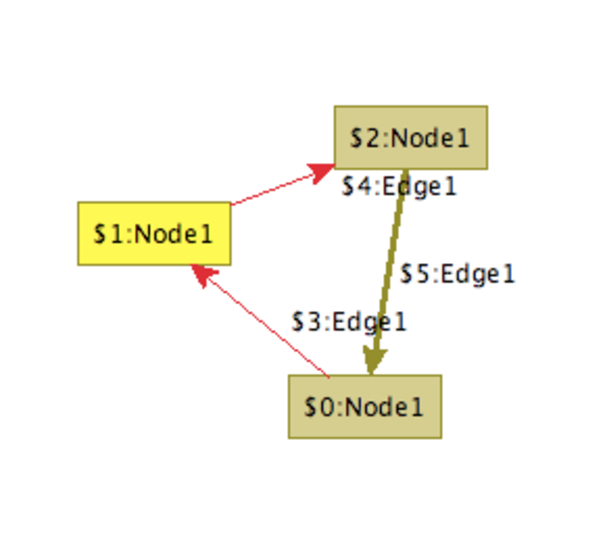
\includegraphics[width=0.25\linewidth]{fig/debug1}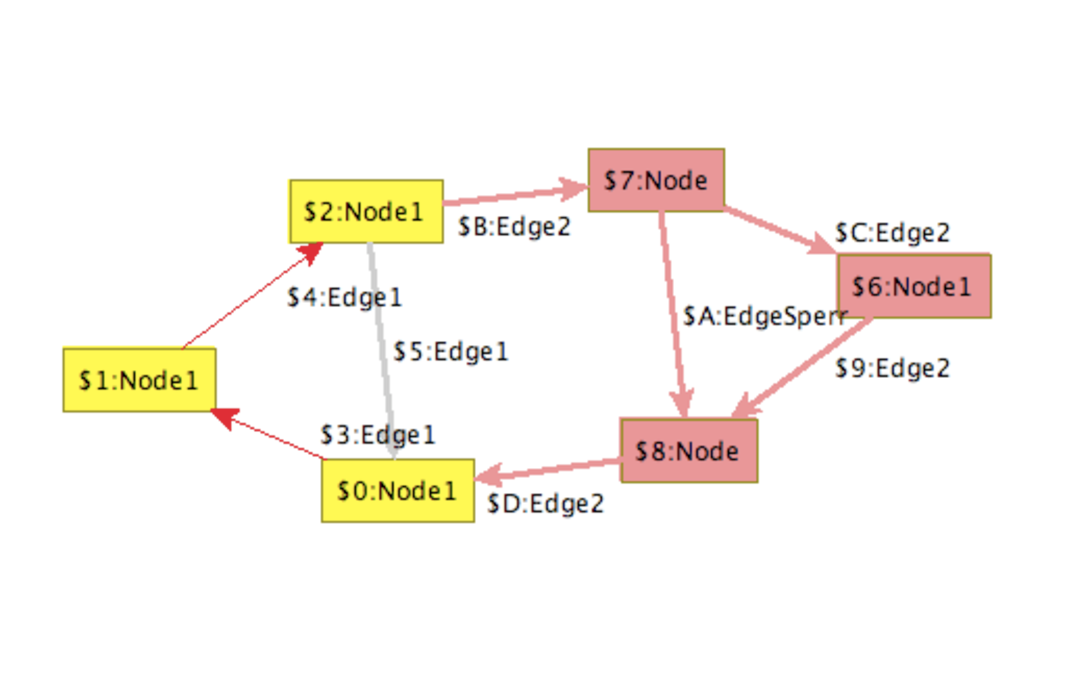
\includegraphics[width=0.4\linewidth]{fig/debug2}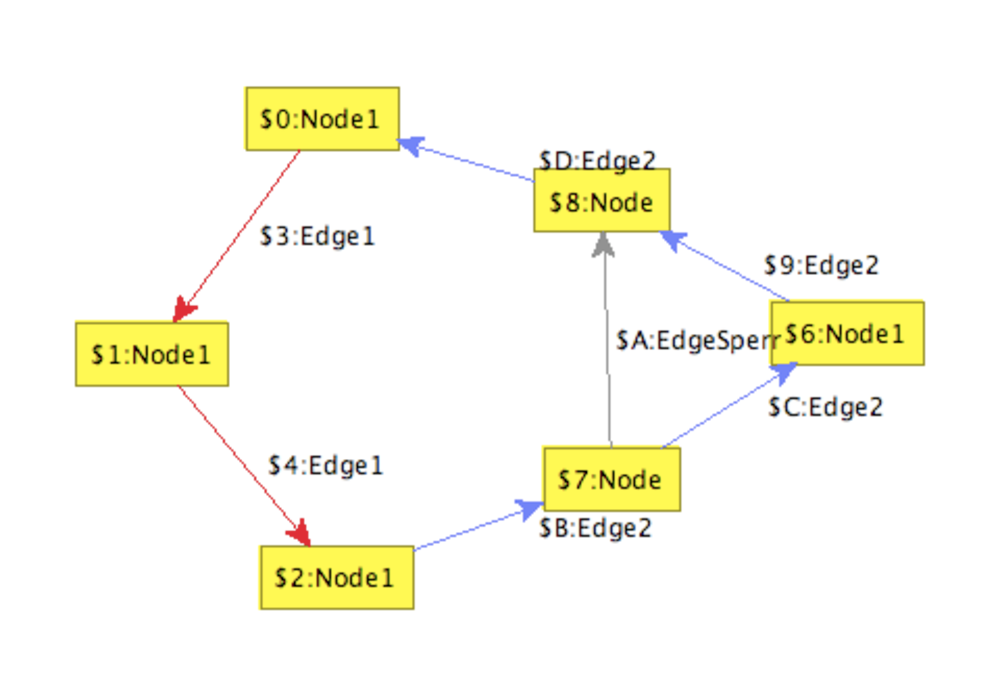
\includegraphics[width=0.4\linewidth]{fig/debug3}
%  \caption{Delayed step rule application.}
%  \label{figdebug}
%\end{figure}

\begin{figure}[htbp]
\begin{example}\label{ex:debug}  
We demonstrate the debug commands with a slightly adjusted script for the Koch snowflake from \GrG's examples (see also Section~\ref{fractals}). The graph rewriting sequence is
\begin{grshell}
debug grs (makeFlake1* ; (beautify ; doNothing)* ; makeFlake2* ; beautify*){1}
\end{grshell}
\yComp\ will be opened with an initial graph (resulting from \texttt{grs init}):
\begin{center}
  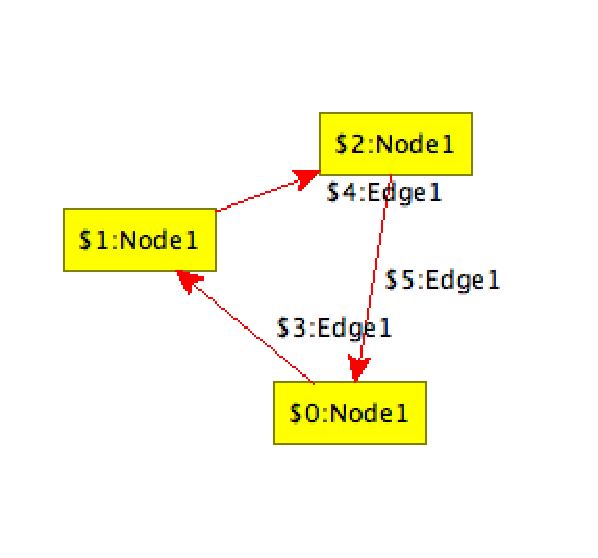
\includegraphics[width=0.3\linewidth]{fig/debug0tra}
\end{center}
We type \texttt{d}(etailed step) to apply \texttt{makeFlake1} step by step resulting in the following graphs:
\begin{center}
  \parbox{0.2\linewidth}{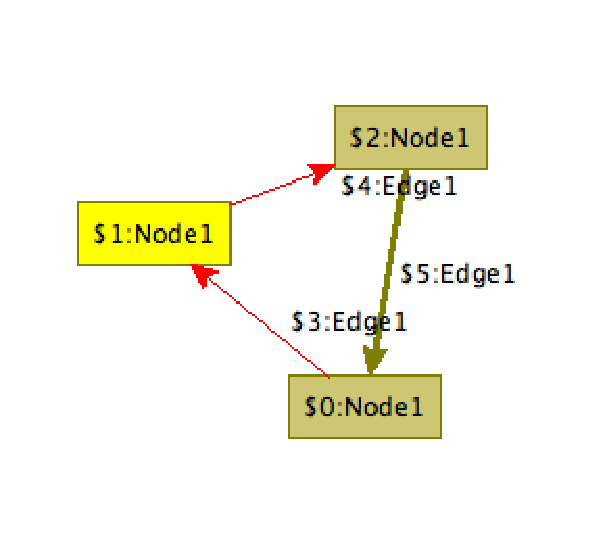
\includegraphics[width=\linewidth]{fig/debug1tra}}\parbox{0.375\linewidth}{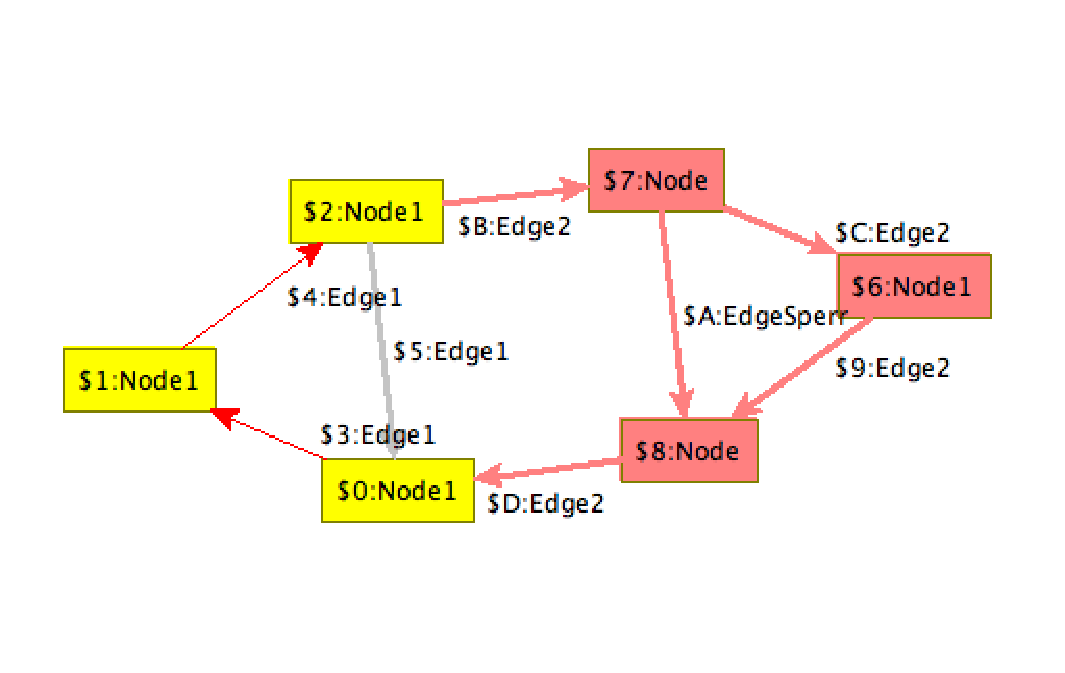
\includegraphics[width=\linewidth]{fig/debug2tra}}\parbox{0.375\linewidth}{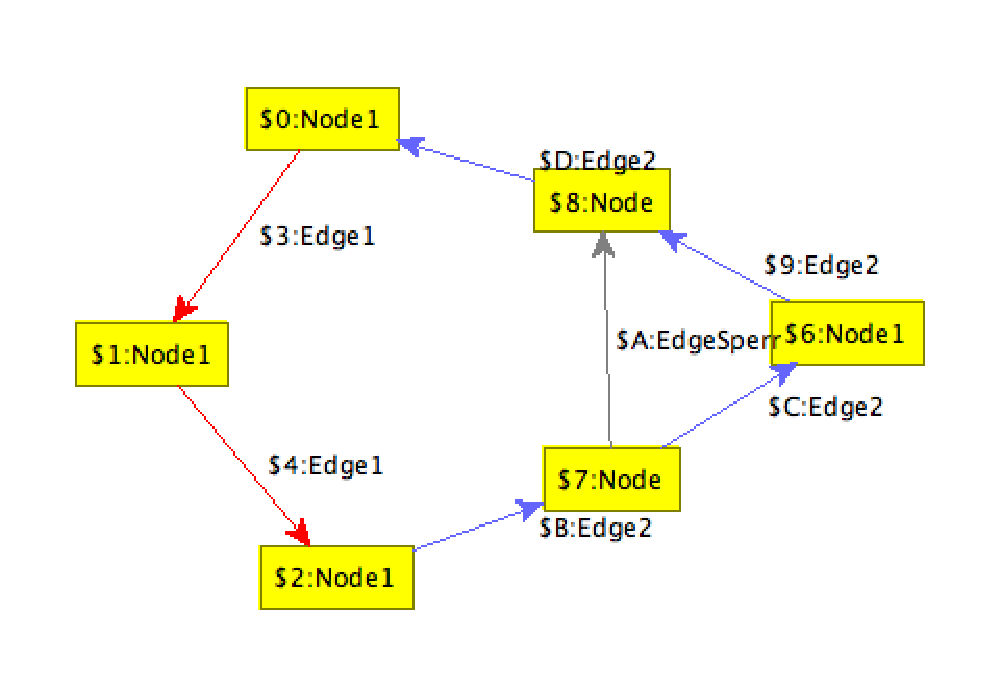
\includegraphics[width=\linewidth]{fig/debug3tra}}
\end{center}
The following table shows the ``break points'' of further debug commands, entered one after another:
\begin{center}
  \begin{tabular}{|l|l|} \hline
    \textbf{Command} & \textbf{Active rule} \\ \hline
    \texttt{s} & \texttt{makeFlake1} \\
    \texttt{o} & \texttt{beautify} \\
    \texttt{s} & \texttt{doNothing} \\
    \texttt{s} & \texttt{beautify} \\ 
    \texttt{n} & \texttt{beautify} \\ 
    \texttt{o} & \texttt{makeFlake2} \\
    \texttt{r} & --- \\ \hline
  \end{tabular}
\end{center}
\end{example}   
\end{figure}


\section{LGSPBackend Custom Commands}
\label{custom}
The \indexed{LGSPBackend} supports the following custom commands:

\subsection{Graph Related Commands}
\begin{rail}
  'custom' 'graph' analyzegraph
\end{rail}\ixkeyw{custom}\ixkeyw{graph}
Analyzes\indexmain{analyzing graph} the current working graph. The analysis data provides vital information for efficient \indexed{search plan}s. Analysis data is available as long as \GrShell\ is running, i.e.\ when the working graph changes, the analysis data is still available but maybe obsolete.

\subsection{Action Related Commands}
\begin{rail}
  'custom' 'actions' gensearchplan (Action+)
\end{rail}\ixkeyw{custom}\ixkeyw{actions}
Creates a search plan for each rewrite rule \emph{Action} using a heuristic method and the analyzes data (if the graph has been analyzed by \texttt{custom graph analyze\_graph}). Otherwise a \indexed{default search plan} is used. For efficiency reasons it is recommended to do analyzing and search plan creation during the rewriting procedure. Therefore the host graph should be in a stage ``similar'' to the final result. Indeed there might be some trial-and-error steps necessary to get an efficient search plan. A search plan is available as long as the current rule set remains loaded. 
Specify multiple rewrite rules instead of using multiple commands for each rule to improve the search plan generation performance.

\begin{rail}
  'custom' 'actions' setmaxmatches Number
\end{rail}\ixkeyw{custom}\ixkeyw{actions}
Sets the maximum amount of possible pattern matches to \emph{Number}. This command affects the expression \texttt{[\emph{Rule}]}. If \emph{Number} is less or equal to zero, the constraint is reset.


